\documentclass[]{article}
\usepackage{lmodern}
\usepackage{amssymb,amsmath}
\usepackage{ifxetex,ifluatex}
\usepackage{fixltx2e} % provides \textsubscript
\ifnum 0\ifxetex 1\fi\ifluatex 1\fi=0 % if pdftex
  \usepackage[T1]{fontenc}
  \usepackage[utf8]{inputenc}
\else % if luatex or xelatex
  \ifxetex
    \usepackage{mathspec}
    \usepackage{xltxtra,xunicode}
  \else
    \usepackage{fontspec}
  \fi
  \defaultfontfeatures{Mapping=tex-text,Scale=MatchLowercase}
  \newcommand{\euro}{€}
\fi
% use upquote if available, for straight quotes in verbatim environments
\IfFileExists{upquote.sty}{\usepackage{upquote}}{}
% use microtype if available
\IfFileExists{microtype.sty}{%
\usepackage{microtype}
\UseMicrotypeSet[protrusion]{basicmath} % disable protrusion for tt fonts
}{}
\usepackage[margin=1in]{geometry}
\usepackage{graphicx}
\makeatletter
\def\maxwidth{\ifdim\Gin@nat@width>\linewidth\linewidth\else\Gin@nat@width\fi}
\def\maxheight{\ifdim\Gin@nat@height>\textheight\textheight\else\Gin@nat@height\fi}
\makeatother
% Scale images if necessary, so that they will not overflow the page
% margins by default, and it is still possible to overwrite the defaults
% using explicit options in \includegraphics[width, height, ...]{}
\setkeys{Gin}{width=\maxwidth,height=\maxheight,keepaspectratio}
\ifxetex
  \usepackage[setpagesize=false, % page size defined by xetex
              unicode=false, % unicode breaks when used with xetex
              xetex]{hyperref}
\else
  \usepackage[unicode=true]{hyperref}
\fi
\hypersetup{breaklinks=true,
            bookmarks=true,
            pdfauthor={},
            pdftitle={Determining the direction of causality in the face of measurement error},
            colorlinks=true,
            citecolor=blue,
            urlcolor=blue,
            linkcolor=magenta,
            pdfborder={0 0 0}}
\urlstyle{same}  % don't use monospace font for urls
\setlength{\parindent}{0pt}
\setlength{\parskip}{6pt plus 2pt minus 1pt}
\setlength{\emergencystretch}{3em}  % prevent overfull lines
\setcounter{secnumdepth}{0}

%%% Use protect on footnotes to avoid problems with footnotes in titles
\let\rmarkdownfootnote\footnote%
\def\footnote{\protect\rmarkdownfootnote}

%%% Change title format to be more compact
\usepackage{titling}

% Create subtitle command for use in maketitle
\newcommand{\subtitle}[1]{
  \posttitle{
    \begin{center}\large#1\end{center}
    }
}

\setlength{\droptitle}{-2em}
  \title{Determining the direction of causality in the face of measurement error}
  \pretitle{\vspace{\droptitle}\centering\huge}
  \posttitle{\par}
  \author{}
  \preauthor{}\postauthor{}
  \predate{\centering\large\emph}
  \postdate{\par}
  \date{14 February 2016}



\begin{document}

\maketitle


Gibran Hemani* and George Davey Smith

MRC Integrative Epidemiology Unit (IEU) at the University of Bristol,
School of Social and Community Medicine, Bristol, UK

* Correspondence to:
\href{mailto:g.hemani@bristol.ac.uk}{\nolinkurl{g.hemani@bristol.ac.uk}}

\subsubsection{Abstract}\label{abstract}

With our ability to characterize the human phenome ever improving it is
becoming increasingly common to use statistical tests to infer the
causal relationships between correlated variables. A simple method for
inferring if an exposure is on the causal pathway to an outcome is
through mediation analysis, where the effect of an instrument on the
outcome is tested before and after adjusting for the exposure. We show
that in the face of measurement error this can lead to erroneous
results, and that increasing sample size, rather than reducing bias, can
often have the alarming effect of increasing certainty in the wrong
answer. Commonly used tools that are predicated on this methodology such
as the causal inference test (CIT) are shown to be susceptible. We
demonstrate that Mendelian randomization (MR) is a method for causal
inference that is robust to measurement error, and that a simple
extension to MR can provide a method to estimate the direction of
causality between correlated variables even when the biology of the
instrument is unknown. We argue that because measurement error is
ubiquitous in phenotypic data, mediation-based causal inference should
be treated with caution.

\subsection{Introduction}\label{introduction}

With the explosion in data that measures the human phenome, of great
interest is understanding the causal nature of the emerging putitive
correlations between measures of interest. Mediation is a commonly used
statistical method for making causal inference in observational
data\textsuperscript{1--4}, and it exists in many forms, from simple
regression based systems to structural equation modeling. The principle
behind mediation analysis can be explained as follows. Supposing an
exposure has a causal effect on an outcome, then an `instrument' that
causes the exposure (a single nucleotide polymorophism (SNP), for
example) should also influence the outcome. Therefore the influence of
the instrument on the outcome conditional on the exposure should be
zero. This forms the basis of a number of methods, such as the causal
inference test (CIT)\textsuperscript{1}, which have been employed by a
number of recent publications make causal inferences, often in large
scale `omics datasets\textsuperscript{5--7}.

While mediation based approaches are simple and convenient to implement,
it is important to note where they may lead to unreliable results. One
such mechanism is measurement error\textsuperscript{8--11}. Measurement
(or observational) error is the difference between a measured value of a
quantity and its true value. Such variability can arise through a whole
plethora of mechanisms, which are often unique to the study design and
difficult to avoid\textsuperscript{12,13}. Array technology is now
commonly used to obtain high throughput phenotyping at low cost, but
they come with the problem of having imperfect sensitivity, so for
example methylation levels as measured by the Illumina450k chip are
prone to have some amount of noise around the true
value\textsuperscript{14,15}. Sensitivity is also an issue, for example
if the unit of measurement of biological interest is the methylation
level in a T cell, then measurement error of this value can be
introduced by using methylation levels from whole blood samples because
the measured value will be an assay of many cell
types\textsuperscript{16}.

Measurement error can indeed arise in more low-tech data too, for
example when measuring body mass index (BMI) one is typically interested
in using this as a proxy for obesity, but it is clear that the
correlation between BMI and obesity is not perfect\textsuperscript{17}.
A similar problem of biological misspecification is unavoidable in
disease diagnosis. Measurement error can also be introduced after the
data has been collected, for example the transformation of non-normal
data for the purpose of statistical analysis will lead to a new variable
that will typically have both bias and imprecision compared to the
original variable. The sources of measurement error are not limited to
this list\textsuperscript{13}, and its impact has been explored in the
context of mediation analysis in the epidemiological literature
extensively\textsuperscript{8,11}.

An alternative statistical method that gained prominence at least in
part as a solution to the problem of measurement
error\textsuperscript{18} is Mendelian randomisation
(MR)\textsuperscript{19,20}. Here an instrumental variable (typically a
SNP) that has a robost, causal association with the exposure is used to
proxy the exposure in an association test with the outcome. If there is
no measurement error in the SNP then the causal association between the
exposure and the outcome can be estimated by scaling the association
between the SNP and the outcome by the association between the SNP and
the exposure. This approach also has the useful property that it guards
against unmeasured confounders driving the association between exposure
and outcome; and if the biological effect of the SNP is understood then
it can also aid against reverse causality driving the association.

Here, however, arises a potential issue. Often the biological effect of
a SNP is not known, and therefore it can be difficult to determine for
which of the two variables in a putative exposure-outcome association is
the SNP a valid instrument. By definition, we expect that if the
association is causal then a SNP for the exposure will be associated
with the outcome, so if the researcher erroneously uses the SNP as an
instrument for the outcome then they are likely to see an apparently
robust causal association of outcome on exposure. Such a situation can
arise in many scenarios. For example genome wide association studies
(GWASs) that identify genetic associations for complex traits are by
design hypothesis free and agnostic of genomic function, and it often
takes years of follow up studies to understand the biological nature of
a putative GWAS hit\textsuperscript{21}. Another situation is where the
causal direction between 'omic measures need to be determined, for
example if a DNA methylation probe is associated with expression of an
adjacent gene, then is a cis-acting SNP an instrument for the DNA
methylation level, or the gene expression level\textsuperscript{7}?

Mediation based methods, for example CIT and other related approaches
typically attempt to use the data to resolve this issue using the
following logic: if the SNP-exposure association is stronger than the
SNP-outcome association then the causal effect must be in the direction
of exposure to outcome. The same logic can indeed be applied to MR, but
often when applied the sensitivity of these approaches to measurement
error is not considered.

When being objective one must assume that measurement error is
ubiquitous, and any measured variable is only an imperfect proxy of the
biological quantity that the researcher intended to obtain. Here we show
using theory and simulations how measurement error can lead to
unreliable causal inference in the mediation-based CIT method, and we
propose an extension to MR that, although does not eliminate the problem
of measurement error, provides a framework in which to ascertain the
causal direction when the biology of the instrument is not fully
understood.

\subsection{Methods}\label{methods}

\subsubsection{CIT test}\label{cit-test}

The CIT method\textsuperscript{1} is implemented in the R package
\emph{R/cit}\textsuperscript{22}. The \emph{cit.cp} function was used to
obtain an omnibus p-value of causality between an exposure \(x\) and an
outcome \(y\) using a mediator \(g\). To infer the direction of
causality using the CIT method, the omnibus p-value was estimated for
\(x\) causing \(y\), and for \(y\) causing \(x\), and the model that
returned the lowest p-value was taken as the one denoting the correct
causal direction.

\subsubsection{MR causal test}\label{mr-causal-test}

Supposing there are two correlated variables, \(x\) and \(y\), with a
variant \(g\) associated with both. Assuming no horizontal pleiotropy
(i.e. \(g\) only has an effect on one of the variables through the other
variable) it is desirable to know which of the variables it has a direct
influence on. This can be achieved by testing for a difference in the
correlations \(\rho_{g, x}\) and \(\rho_{g, y}\) using Steiger's Z-test
for correlated correlations within a
population\textsuperscript{\textbf{???}}. It is calculated as

\[
Z = (Z_{gx} - Z_{gy}) \frac{\sqrt{N-3}}{\sqrt{2(1-\rho_{xy})h}}
\]

where Fisher's z-transformation is used to obtain
\(Z_{g*} = \frac{1}{2} \ln \left ( \frac{1+\rho_{g*}}{1-\rho_{g*}} \right )\),

\[
h = \frac{1 - (frm^2)} {1 - rm^2}
\]

where

\[
f = \frac{1 - \rho_{xy}}{2(1 - rm^2)}
\]

and

\[
rm^2 = \frac{1}{2}(\rho_{gx}^2 + \rho_{gy}^2).
\]

The \(Z\) value is interpreted such that

\[
Z \left\{
\begin{array}{ll}
> 0, & x \to y\\
< 0, & y \to x\\
= 0, & x \perp\!\!\!\perp y 
\end{array} \right.
\]

and a p-value is generated from the \(Z\) value to indicate confidence
of difference in correlations \(\rho_{gx}\) and \(\rho_{gy}\). The test
for a causal association is then obtained by performing two sample MR in
the direction that is predicted to be the correct model based on the Z
score test. For simplicity, the test is deemed to have obtained a robust
association if the Z score test has a p-value \(< 0.05\) and the two
sample MR analysis has a p-value \(< 0.05\). Note that the same approach
can be applied to a two-sample MR setting, where

\subsubsection{Simulations}\label{simulations}

Simulations were conducting by creating variables of sample size \(n\)
for the exposure \(x\), the measured values of the exposure \(x_O\), the
outcome \(y\), the measured values of the outcome \(y_O\) and the
instrument \(g\). In all models \(x\) causes \(y\) and \(g\) is an
instrument for \(x\). Each variable was simulated such that:

\[
\begin{aligned}
g & \sim Binom(2, 0.5) \\
x & = \beta_g g + \epsilon_g \\
x_O & = \beta_{mx} x + \epsilon_{mx} \\
y & = \beta_x x + \epsilon_x \\
y_O & = \beta_{my} y + \epsilon_{my} \\
\end{aligned}
\]

All \(\beta\) values were set to 1. Values of \(\epsilon_*\) were
generated such that

\[
\begin{aligned}
cor(g, x) & = \{0.01, 0.05, 0.1\} \\
cor(x, y) & = \{0.2, 0.4, 0.6, 0.8\} \\
var(\epsilon_{mx}) & = \{0, 0.2, 0.4, 0.6, 0.8, 1\} \\
var(\epsilon_{my}) & = \{0, 0.2, 0.4, 0.6, 0.8, 1\} \\
n & = \{100, 1000, 10000\}
\end{aligned}
\]

giving a total of 432 combinations of parameters. Each of these sets of
variables was performed 100 times, and the CIT and MR methods were
applied to each in order to evaluate the causal association of the
simualted variables.

\subsection{Results}\label{results}

\subsubsection{The influence of measurement error on
CIT}\label{the-influence-of-measurement-error-on-cit}

Measurement error of an exposure can be modeled as some transformation
of the true value that leads to the observed value, \(x_O=f(x)\). For
example, we can define \(f(x) = \alpha_m + \beta_m x + \epsilon_m\),
where \(\alpha_m\) and \(\beta_m\) influence the bias in the measurement
of \(x\), and \(\epsilon_m\) represents the imprecision in the
measurement of \(x\). Here the true value of the exposure is partially
explained by the genetic instrument, \(g\), such that

\[
x = \alpha_g + \beta_g g + \epsilon_g
\]

where \(\beta_g\) is the effect of the SNP on the exposure, and
\(\epsilon_g\) is the residual value of \(x\); and the outcome is
partially explained by the exposure

\[
y = \alpha_x + \beta_x x + \epsilon_x
\]

where \(\beta_x\) is the true effect of the exposure on the outcome. In
the causal inference test (CIT), an omnibus p-value is generated from
four hypothesis tests: 1) \(g\) is associated with \(x\); 2) \(g\) is
associated with \(y\); 3) \(g\) is associated with \(x|y\); and 4) \(g\)
is independent of \(y|x\). The 4th condition is necessary for causal
inference, and can be expressed as \(cov(g, y - \hat{y}) = 0\), where
\(\hat{y} = \hat{\alpha}_x + \hat{\beta}_x x_O\). When measurement error
is introduced we can show using basic covariance properties (Appendix 1)
that

\[
\begin{aligned}
cov(g, y - \hat{y}) & = cov(g, y) - cov(g, \hat{y})  \\
                    & = \beta_g \beta_x var(g) - D\beta_g \beta_x var(g)
\end{aligned}
\]

where

\[
D = \frac{\beta^2_m var(x)} {\beta^2_m var(x) + var(\epsilon_m)}
\]

Thus an observational study will find \(cov(g, y - \hat{y}) = 0\) when
the true model is causal only when \(D = 1\). Therefore, if there is any
measurement error that incurs imprecision (i.e.
\(var(\epsilon_m) \neq 0\)) then there will remain an association
between \(g\) and \(y|x\), which is in violation of the the 4th
condition of the CIT. Note that measurement bias alone is insufficient
to lead to a violation of the test statistic assumptions.

We performed simulations to verify that this problem does arise using
the CIT method. Figure 1 shows that when there is no measurement error
in the exposure or outcome variables (\(\rho_{x, x_O}=1\)) the CIT is
reliable in identifying the correct causal direction. However, as
measurement error increases in the exposure variable, eventually the CIT
is more likely to infer a robust causal association in the wrong
direction. Also of concern here is that increasing sample size does not
solve the issue, indeed it only strengthens the evidence of the
incorrect inference.

\subsubsection{Inferring direction of causality using
MR}\label{inferring-direction-of-causality-using-mr}

When selecting an instrument \(g\) that has a direct influence on \(x\)
and \(x\) is causally related to \(y\), one can reason that the
influence of \(g\) on \(y\) is the proportion of the effect of \(x\) on
\(y\) that is explained by the effect of \(g\) on \(x\). Hence the
effect estimate \(\beta_{MR}\) of \(x\) on \(y\) is estimated as

\[
\beta_{MR} = \frac{\beta_y}{\beta_g} = \frac{cov(y, g)}{cov(x_O, g)} = \frac{cov(\beta_x x + \epsilon_x, g)}{cov(x + \epsilon_x, g)}
\]

which reduces to

\[
\lim_{n \to \infty} \hat{\beta}_{MR} = \frac{\beta_x cov(x + \epsilon_x)}{cov(x + \epsilon_x)} = \beta_x
\]

thus we obtain an estimate of the effect of \(x_O\) on \(y\) that is
unbiased by measurement error in \(x\).

However, if we do not know whether the SNP \(g\) has a direct influence
on \(x\) or \(y\) then further efforts are required. If \(x\) causes
\(y\) and \(g\) is a valid instrument for \(x\) then we expect that the
Steiger test will obtain the correct result because the value
\(d = \rho_{g, x_O} - \rho_{g, y_O}\) is greater than 0 when the causal
association between \(x\) and \(y\) is \(\rho_{x, y} < 1\). But it can
be shown that in the presence of measurement error,
\(d = \rho_{x, x_O} - \rho_{x,y}\rho_{y,y_O}\) (Appendix 2), thus it is
important to note that under certain conditions when measurement error
is present the Steiger test could make erroneous inference about causal
direction because the value of \(d\) is not restricted to being greater
than 0. However, using the MR approach there are two potential
advantages over the CIT. First, we can conduct a formal test for the
direction of causality. Second the correct direction of causality can be
inferred when measurement error in the exposure variable is present, as
long as it is lower than the product of the measurement error in the
outcome and the causal correlation between the exposure and the outcome.
Figure 2 shows that in most cases, especially when the causal effect
between \(x\) and \(y\) is not very large, the condition of \(d > 0\) is
satisfied.

We performed simulations to explore the performance of this approach in
comparison to CIT. Figure 3 shows that, as predicted, when \(d < 0\) the
MR analysis is liable to infer the wrong direction of causality, and
that this erroneous result is more likely to occur with increasing
sample size. However, in all cases the MR analysis infers the wrong
direction of causality at the same or a lower rate than the CIT. When
\(d > 0\) is satisfied we observe that in many cases the MR method has
greater power to obtain evidence for causality than CIT, and always
obtains the correct direction of causality.

\subsection{Discussion}\label{discussion}

Researchers are often confronted with the problem of making causal
inferences using a statistical framework on observational data, and
unfortunately there are no solutions that work perfectly in all
scenarios. In the face of measurement error it is evident that causal
inference drawn through mediation analysis will be difficult to
interpret, and this is a serious problem considering that it is often
impossible to estimate the extent of measurement error for most
experimental designs.

In the epidemiological literature this is relatively well understood and
our initial analysis simply confirms that for widely used methods such
as CIT that it is indeed liable to the same issues as standard mediation
based analysis. Under many circumstances a practical solution to this
problem is to use Mendelian randomisation instead of mediation based
methods. Mendelian randomisation is robust in the face of measurement
error and, given that the researcher has knowledge about the biology of
the instrument being used in the analysis, can offer a direct solution
to the issues that CIT faces. This assumption is often reasonable, for
example exposures such as CRP

Pleiotropy

\subsection{Appendix 1}\label{appendix-1}

Given the following model

\[
x = \alpha_g + \beta_g g + \epsilon_g \\
x_O = \alpha_m + \beta_m x + \epsilon_m \\
y = \alpha_x + \beta_x x + \epsilon_x
\]

where \(x\) is the exposure on the outcome \(y\), \(g\) is an instrument
that has a direct effect on \(x\), and \(x_O\) is the measured quantity
of \(x\), where measurement error is incurred from bias in \(\alpha_m\)
and \(\beta_m\) and imprecision from \(\epsilon_m\), our objective is to
estimate the expected magnitude of association between \(g\) and \(y\)
after conditioning on \(x\). Under the CIT, this is expected to be
\(cov(g, y - \hat{y}) = 0\) when \(x\) causes \(y\), where
\(\hat{y} = \hat{a}_{x_O} + \hat{b}_{x_O} x_O + \epsilon_{x_O}\) is the
predicted value of \(y\) using the measured value of \(x_O\).

We can split \(cov(g, y - \hat{y})\) into two parts, \(cov(g, y)\) and
\(cov(g, \hat{y})\).

\textbf{Part 1}

\[
\begin{aligned}
cov(g, y) & = cov(g, \beta_x x) \\
          & = cov(g, \beta_x \beta_g g) \\
          & = \beta_x\beta_g var(g)
\end{aligned}
\]

\textbf{Part 2}

\[
\begin{aligned}
cov(g, \hat{y}) & = cov(g, \hat{\beta}_{x_O} x_O) \\
                & = cov(g, \hat{\beta}_{x_O} \beta_m x) \\
                & = cov(g, \hat{\beta}_{x_O} \beta_m \beta_g g) \\
                & = \hat{\beta}_{x_O} \beta_m \beta_g var(g)
\end{aligned}
\]

Simpifying further

\[
\begin{aligned}
\hat{\beta}_{x_O} & = \frac{cov(y, x_O)} {var(x_O)} \\
                  & = \frac{\beta_m cov(y, x)} {var(x_O)} \\
                  & = \frac{\beta_m \beta_x var(x)} {var(x_O)} \\
                  & = \frac{\beta_m \beta_x var(x)} {\beta_m^2 var(x) + var(\epsilon_m)}
\end{aligned}
\]

which can be substituted back to give

\[
\begin{aligned}
cov(g, \hat{y}) & = \frac{\beta_x\beta_g var(g) \beta_m^2 var(x)} {\beta_m^2 var(x) + var(\epsilon_m)} \\
                & = D\beta_x\beta_g var(g)
\end{aligned}
\]

where

\[
D = \frac{\beta_m^2 var(x)} {\beta_m^2 var(x) + var(\epsilon_m)}
\]

\subsection{Appendix 2}\label{appendix-2}

Steiger test is used to infer if the variant \(g\) has a direct
influence on \(x\) or \(y\) when it is known that it associates with
both, but the direction of causality between \(x\) and \(y\) is unknown.
Assuming the causal direction is \(x \to y\), two stage MR is formulated
using the following regression models:

\[
x = \alpha_1 + \beta_1 g + e_1
\]

for the first stage and

\[
y = \alpha_2 + \beta_2 \hat{x} + e_2
\]

where \(\hat{x} = \hat{alpha}_1 + \hat{\beta}_1 g\). Writing in scale
free terms, \(\rho_{g, x}\) denotes the correlation between \(g\) and
the exposure variable \(x\), and it is expected that
\(\rho_{g, x} > \rho_{g, y}\) because
\(\rho_{g, y} = \rho_{g, x}\rho_{x, y}\), where \(\rho_{x, y}\) is the
causal association between \(x\) and \(y\) (which is likely to be less
than 1). In the presence of measurement error in \(x\) and \(y\),
however, Steiger test will instead be assessing the inequality
\(\rho_{g, x_O} > \rho_{g, y_O}\), which can be simplified:

\[
\begin{aligned}
\rho_{g, x_O} & > \rho_{g, y_O} \\
\rho_{g, x} \rho_{x, x_O} & > \rho_{g,y}\rho_{y,y_O}\\
\rho_{g, x} \rho_{x, x_O} & > \rho_{g,x}\rho_{x,y}\rho_{y,y_O}\\
\rho_{x, x_O} & > \rho_{x,y}\rho_{y,y_O}
\end{aligned}
\]

\newpage

\subsection{Tables}\label{tables}

\newpage

\subsection{Figures}\label{figures}

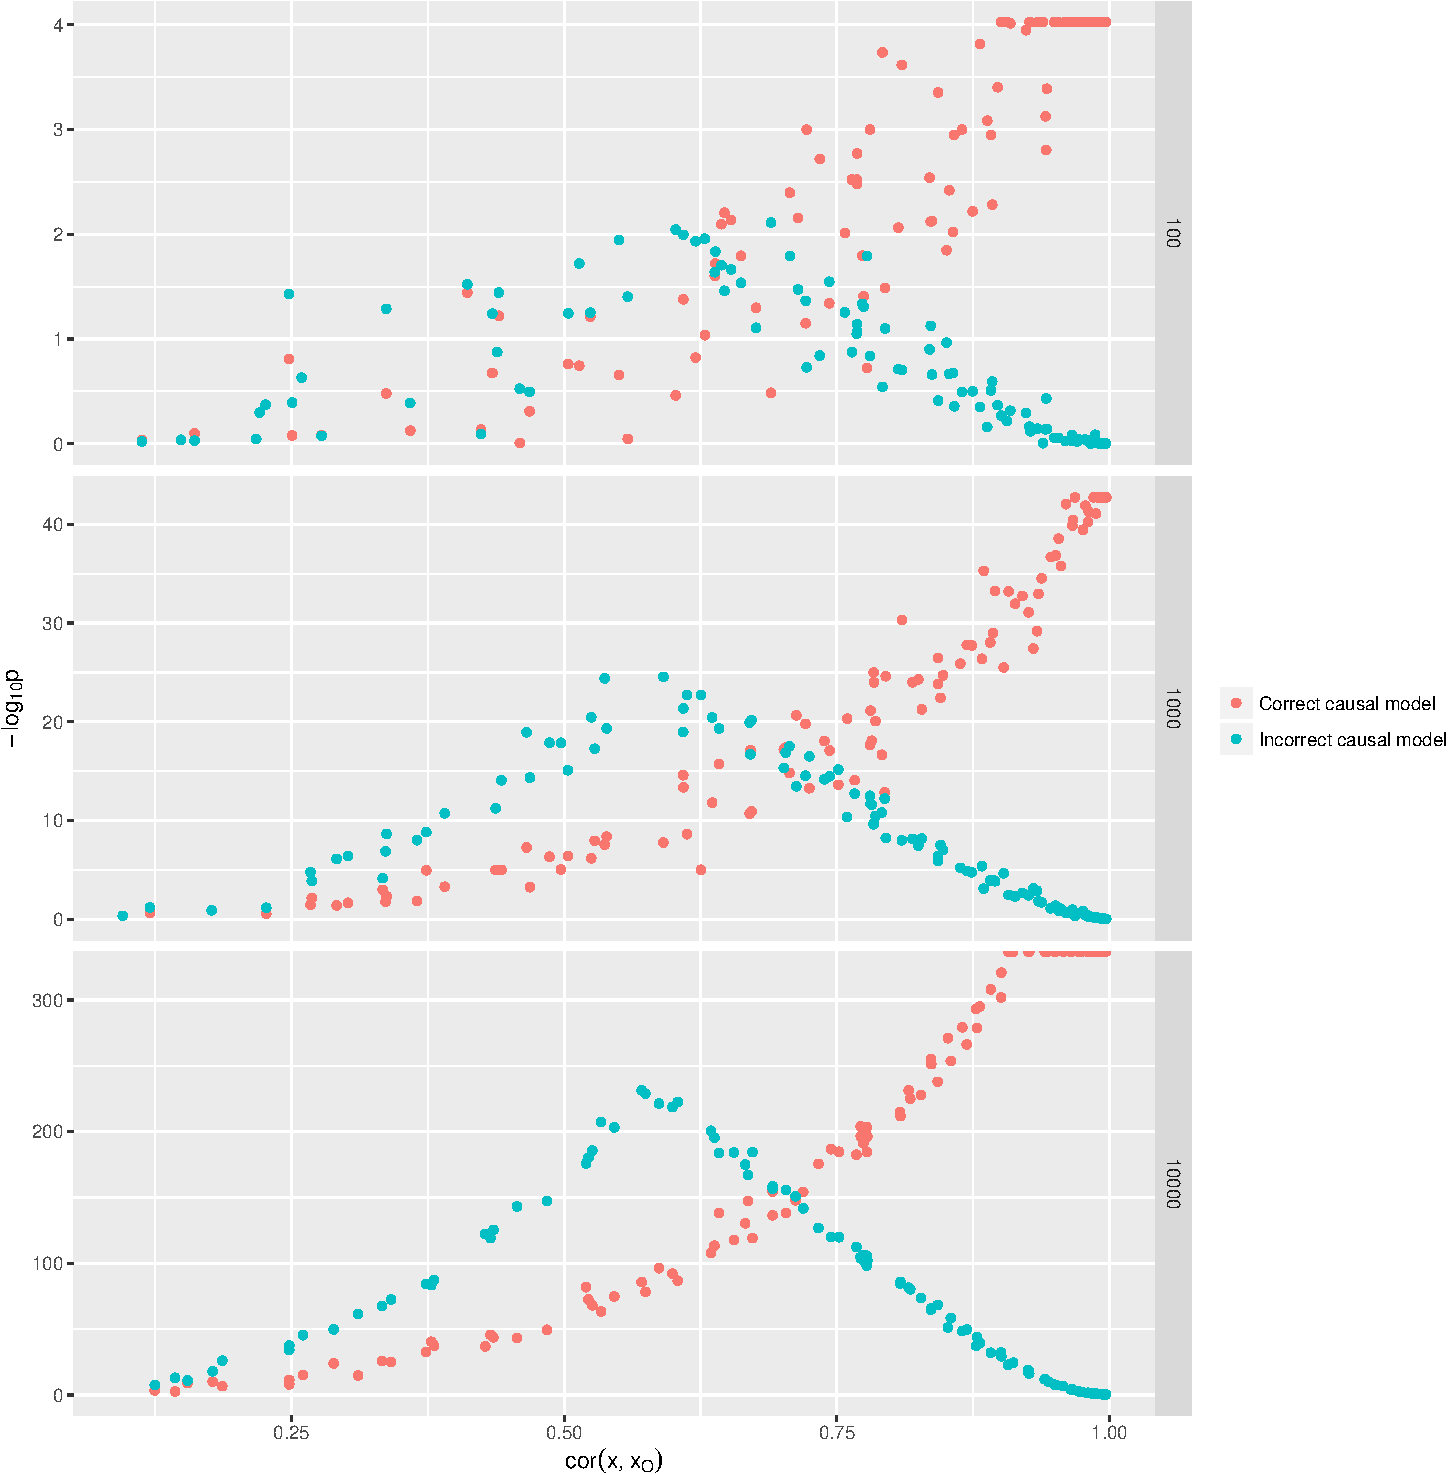
\includegraphics{manuscript_files/figure-latex/cit_measurement_error_figure-1.pdf}\\
Figure 1: The CIT was performed on simulated variables where the
exposure influenced the outcome and the exposure was instrumented by a
SNP. The test statistic from CIT when testing if the exposure caused the
outcome (the true model) is in red, and the test for the outcome causing
the exposure (false model) is in green. Rows of plots represent the
sample sizes used for the simulations. As measurement error increases
(decreasing values on x-axis) the test statistic for the incorrect model
gets stronger and the test statistic for the correct model gets weaker.

\newpage

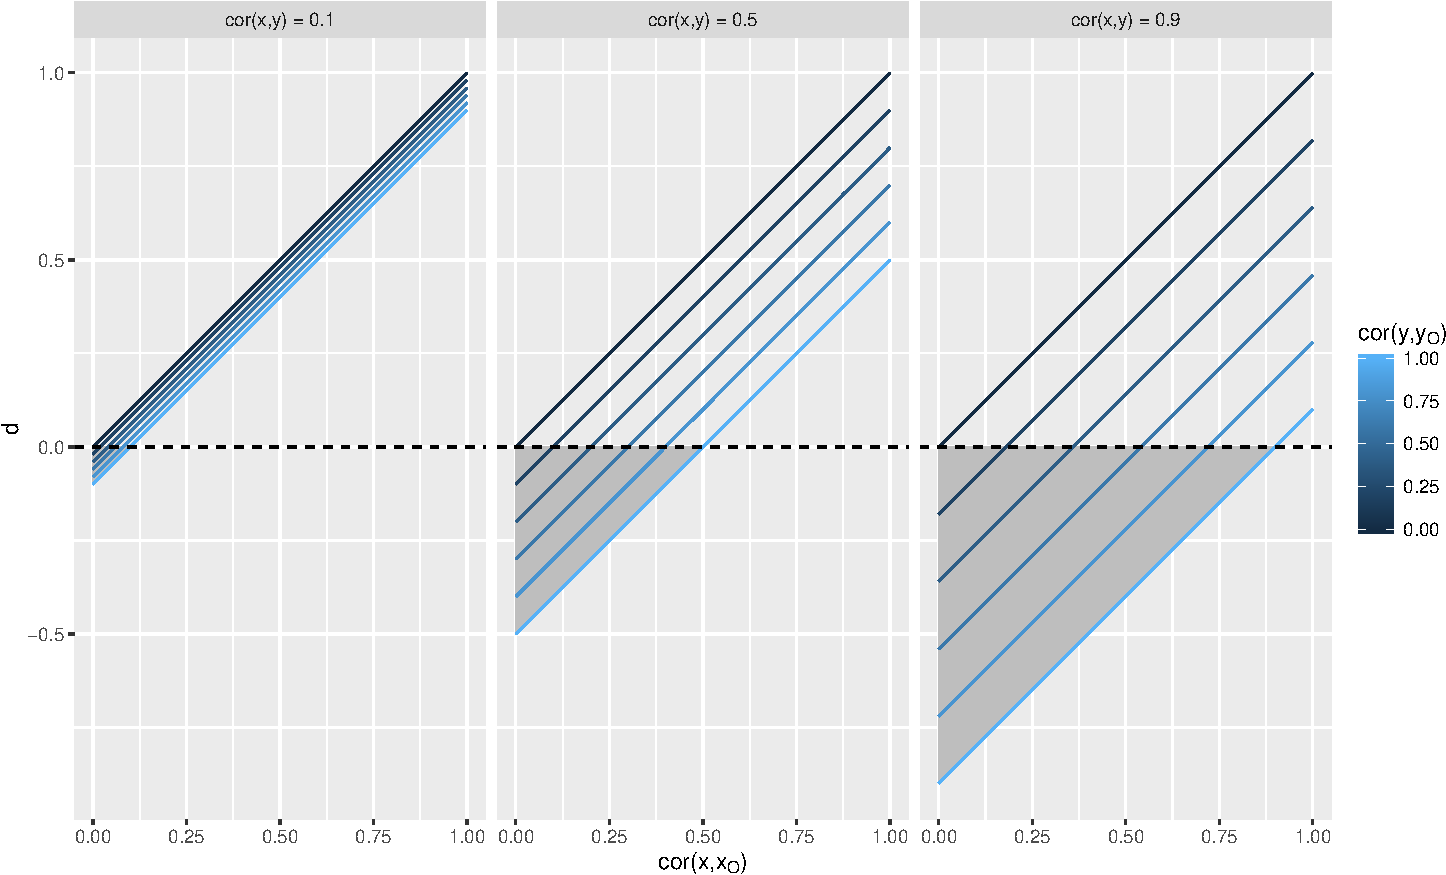
\includegraphics{manuscript_files/figure-latex/d_relationship_figure-1.pdf}\\
Figure 2: Plots depicting the function
\(d = cor(x, x_O) - cor(x,y)cor(y, y_O)\).

\newpage

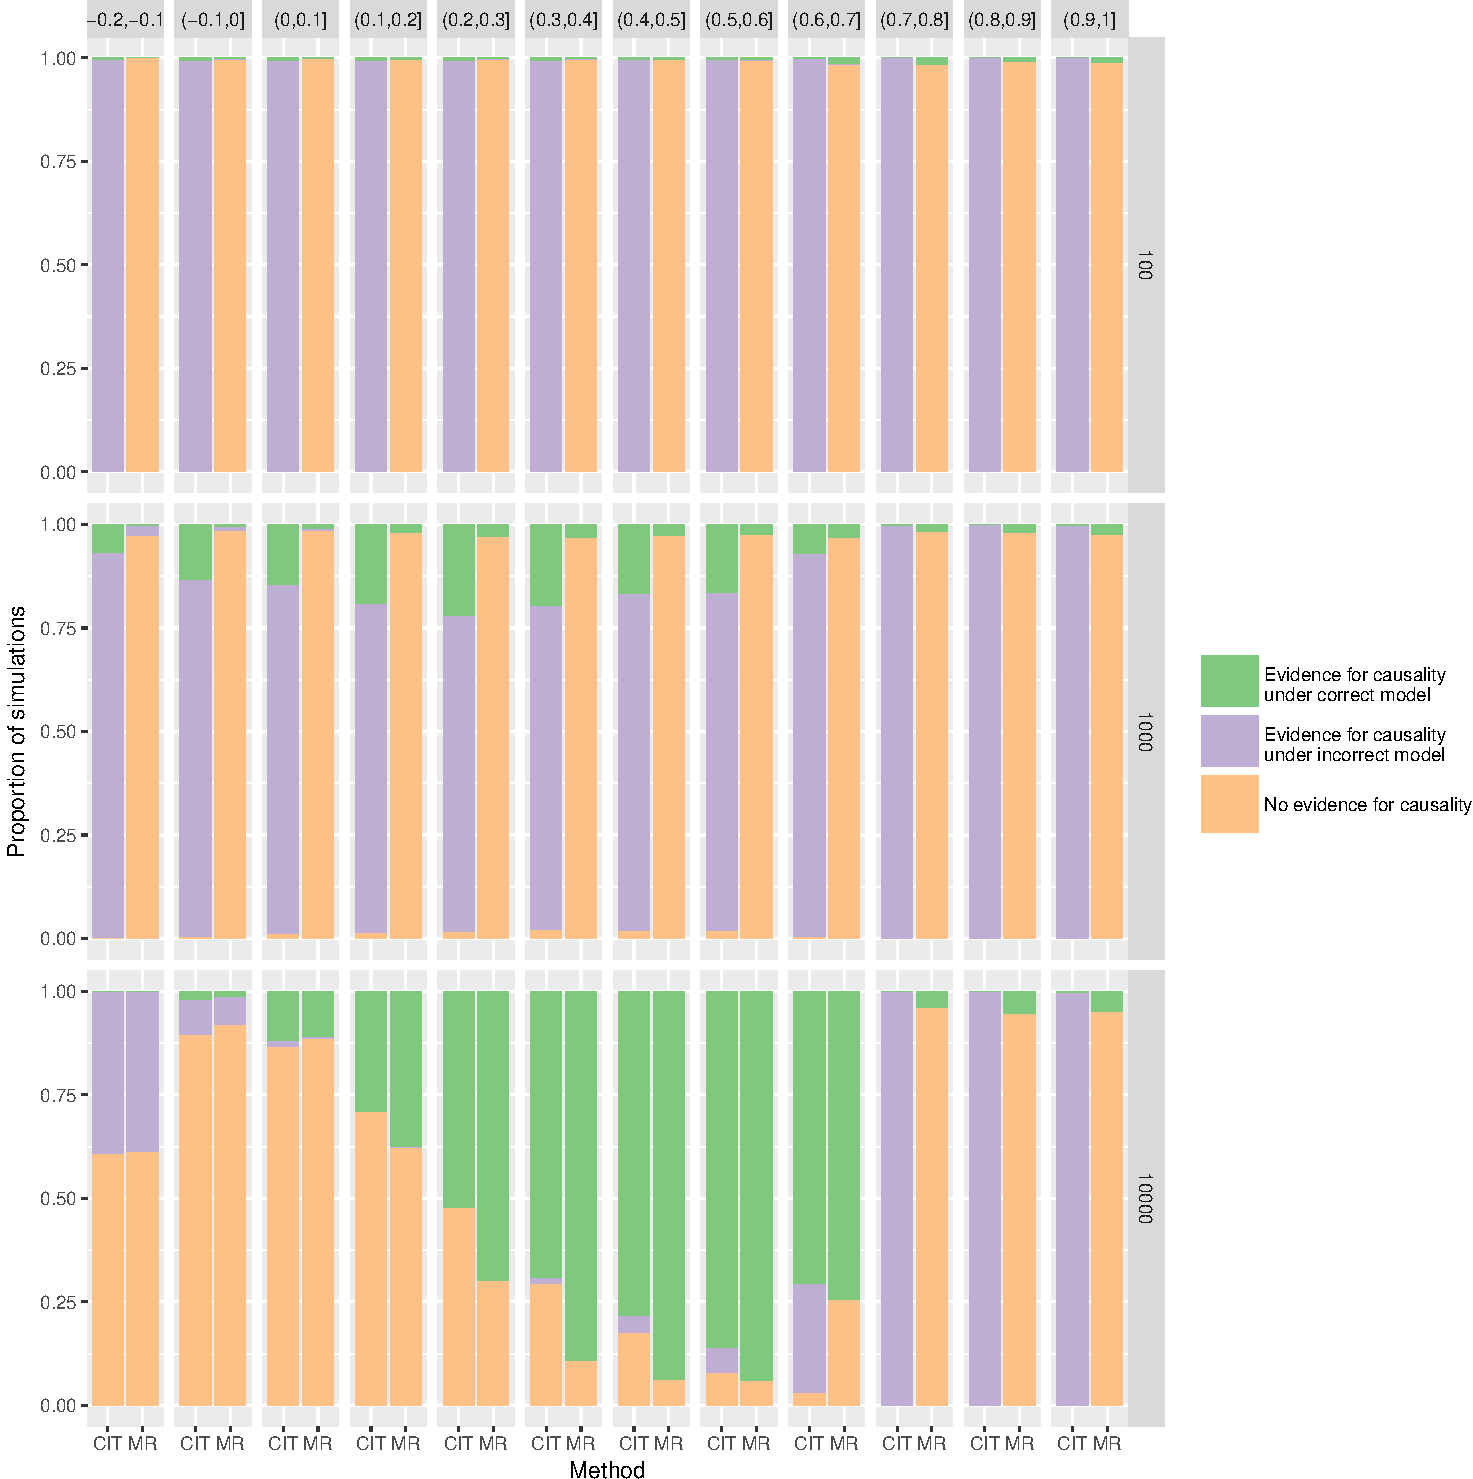
\includegraphics{manuscript_files/figure-latex/cit_mr_comparison_figure-1.pdf}\\
Figure 3: Outcomes were simulated to be causally influenced by
exposures, with varying degrees of measurement error applied to both.
CIT and MR were used to infer evidence for causality between the
exposure and outcome, and to infer the direction of causality. The value
of \(d = \rho_{x, x_O} - \rho_{x,y}\rho_{y,y_O}\), such that when \(d\)
is negative we expect the Steiger test to be more likely to be wrong
about the direction of causality. Rows of graphs represent the sample
size used in the simulations.

\newpage

\subsection{Supplementary tables}\label{supplementary-tables}

\newpage

\subsection{Supplementary figures}\label{supplementary-figures}

\subsection*{References}\label{references}
\addcontentsline{toc}{subsection}{References}

1.Millstein, J., Zhang, B., Zhu, J. \& Schadt, E. E. Disentangling
molecular relationships with a causal inference test. \emph{BMC
genetics} \textbf{10,} 23 (2009).

2.Schadt, E. E. \emph{et al.} An integrative genomics approach to infer
causal associations between gene expression and disease. \emph{Nature
Genetics} \textbf{37,} 710--717 (2005).

3.Gayan, J., Gonzalez-Perez, A. \& Ruiz, A. `Does replication groups
scoring reduce false positive rate in SNP interaction discovery?
Response'. \emph{BMC Genomics} \textbf{11,} 403 (2010).

4.Tavtigian, S. V. \emph{et al.} Rare, Evolutionarily Unlikely Missense
Substitutions in ATM Confer Increased Risk of Breast Cancer. \emph{The
American Journal of Human Genetics} \textbf{85,} 427--446 (2009).

5.Koestler, D. C. \emph{et al.} Integrative genomic analysis identifies
epigenetic marks that mediate genetic risk for epithelial ovarian
cancer. \emph{BMC medical genomics} \textbf{7,} 8 (2014).

6.Liu, Y. \emph{et al.} Epigenome-wide association data implicate DNA
methylation as an intermediary of genetic risk in rheumatoid arthritis.
\emph{Nature biotechnology} \textbf{31,} 142--7 (2013).

7.Waszak, S. M. \emph{et al.} Variation and genetic control of chromatin
architecture in humans. \emph{Cell} \textbf{162,} 1039--1050 (2015).

8.Cessie, S. le, Debeij, J., Rosendaal, F. R., Cannegieter, S. C. \&
Vandenbroucke, J. P. Quantification of bias in direct effects estimates
due to different types of measurement error in the mediator.
\emph{Epidemiology (Cambridge, Mass.)} \textbf{23,} 551--60 (2012).

9.Nagarajan, R. \& Scutari, M. Impact of noise on molecular network
inference. \emph{PloS one} \textbf{8,} e80735 (2013).

10.Shpitser, I., VanderWeele, T. \& Robins, J. On the validity of
covariate adjustment for estimating causal effects. \emph{Proceedings of
the Twenty Sixth Conference on Uncertainty in Artificial Intelligence
(UAI-10)} 527--536 (2010).

11.Blakely, T., McKenzie, S. \& Carter, K. Misclassification of the
mediator matters when estimating indirect effects. \emph{Journal of
epidemiology and community health} \textbf{67,} 458--66 (2013).

12.Houle, D., P{é}labon, C., Wagner, G. \& Hansen, T. Measurement and
meaning in biology. \emph{The Quarterly Review of Biology} \textbf{86,}
3--34 (2011).

13.Hern{á}n, M. a \& Cole, S. R. Invited Commentary: Causal diagrams and
measurement bias. \emph{American journal of epidemiology} \textbf{170,}
959--62; discussion 963--4 (2009).

14.Harper, K. N., Peters, B. a \& Gamble, M. V. Batch effects and
pathway analysis: two potential perils in cancer studies involving DNA
methylation array analysis. \emph{Cancer epidemiology, biomarkers \&
prevention : a publication of the American Association for Cancer
Research, cosponsored by the American Society of Preventive Oncology}
\textbf{22,} 1052--60 (2013).

15.Chen, Y.-a. \emph{et al.} Discovery of cross-reactive probes and
polymorphic CpGs in the Illumina Infinium HumanMethylation450
microarray. \emph{Epigenetics : official journal of the DNA Methylation
Society} \textbf{8,} 203--9 (2013).

16.Houseman, E. A. \emph{et al.} DNA methylation arrays as surrogate
measures of cell mixture distribution. \emph{BMC bioinformatics}
\textbf{13,} 86 (2012).

17.Ahima, R. S. \& Lazar, M. A. Physiology. The health risk of
obesity--better metrics imperative. \emph{Science (New York, N.Y.)}
\textbf{341,} 856--8 (2013).

18.Ashenfelter, O. \& Krueger, A. B. Estimates of the Economic Return to
Schooling from a New Sample of Twins. \emph{The American Economic
Review} \textbf{84,} 1157--1173 (1994).

19.{Davey Smith}, G. \& Ebrahim, S. Mendelian randomization: prospects,
potentials, and limitations. \emph{International journal of
epidemiology} \textbf{33,} 30--42 (2004).

20.{Davey Smith}, G. \& Hemani, G. Mendelian randomization: genetic
anchors for causal inference in epidemiological studies. \emph{Human
molecular genetics} \textbf{23,} R89-----R98 (2014).

21.Claussnitzer, M. \emph{et al.} FTO Obesity Variant Circuitry and
Adipocyte Browning in Humans. \emph{The New England journal of medicine}
\textbf{373,} 895--907 (2015).

22.Millstein, J. \emph{cit: Causal Inference Test}. (2016). at
\textless{}\url{http://cran.r-project.org/package=cit}\textgreater{}

\end{document}
